%%%%%%%%%%%%%%%%%%%%%%%%%%%%%%%%%%%%%%%%%%%%%%%%%%%%%%

In this chapter, the experimental evaluation of MOEA/D will be introduce. In order to achieve an accurate comparison of MOEA/D with the results obtained in \cite{Miranda2018} by other algorithms mentioned before (NSGA-II and SPEA-2), the algorithm and the experimental evaluation were development through the same framework used in \cite{Miranda2018} called Metaheuristic-based Extensible Tool for Cooperative Optimisation (METCO)~\footnote{Available at: https://github.com/PAL-ULL/software-metco} proposed in \cite{METCO}.
In addition, the experiment were executed on a Debian GNU/Linux computer with four AMD Opteron processors at 2.8GHz and 64 GB RAM and each run was repeated 25 times.
Furthermore, following the evaluation procedure done by the authors in \cite{Miranda2018}, the \textit{hypervolume~(HV)}~\cite{HYPER} was the metric selected to compare the different configurations of MOEA/D and the \textit{Shapiro-Wilk, Levene, ANOVA or Welch} test were considered for results which follow a normal distribution or \textit{Kruskal-Wallis} test otherwise. However, in this Master Thesis the number of individual evaluations was decreased from 4e8 evaluations to 1e8 evaluations in order to obtain the results in a faster way.
%%%%%%%%%%%%%%%%%%%%%%%%%%%%%%%%%%%%%%%%%%%%%%%%%%%%%%%%
\section{Instances}
For this evaluation, a total number of 67 different courses were available group together in three different files:
\begin{itemize}
    \item $l_{st}$: 19 starters.
    \item $l_{mc}$: 34 main courses.
    \item $l_{ds}$: 14 desserts.
\end{itemize}
Besides, the structure of every file is an CSV file with the following fields:
\begin{itemize}
    \item Name of the course.
    \item Price of the course.
    \item Binary list of different allergens in case whether the course contains or not the allergen.
    \item Incompatibilities.
    \item Amount of the different nutrients.
    \item Food groups which belongs the course.
\end{itemize}
%%%%%%%%%%%%%%%%%%%%%%%%%%%%%%%%%%%%%%%%%%%%%%%
\section{Parameter Setting}
In this preliminary experiment, the main goal was to find which values of the MOEA/D\cite{Zhang2007} parameters form the better configuration facing the MPP formulation considered in this Master Thesis. The list of MOEA/D's parameters is:
\begin{itemize}
    \item Population size.
    \item Neighbourhood size.
    \item Mutation probability that was set at 0.05.
    \item Crossover probability which was set at 1.
\end{itemize}
At this point, it must be say that MPP takes one parameter which defines the number of different days that in this preliminary experiment was set at \textbf{20 days}. 
The comments of the MOEA/D's authors in \cite{Zhang2007} about the performance of the algorithm with very small or large neighbourhood size and the effect of the population size on its performance were took into account when designing this experiment. However, a wide range of values were considered. Then, five different values for the population size and neighbourhood size were set in order to obtain 25 different configurations of MOEA/D. The values are:
\begin{itemize}
    \item Population size: 25, 80, 140, 190, 250.
    \item Neighbourhood size: 0.4, 0.3, 0.25, 0.2, 0.16 percentage of the total population size.
\end{itemize}
Table \ref{ranking} shows the ranking of all MOEA/D configuration for a 20-days MPP related to the hypervolume values obtained at the end of the executions. The ranking \textit{(R)} was calculated considering the number of times that one configuration outperforms other configurations \textit{(W)} and the number of times that it was outperformed by other configurations \textit{(L)}: 
\[ 
R = W - L
\]
Configuration A statistically outperforms configuration B if the p-value, obtained after performing a pairwise comparison of both approaches by following the statistical testing procedure described at the beginning of this chapter, is lower than the significance level $\alpha = 0.05$ , and if at the same time, A provides a higher mean and median of the hypervolume at the end of the runs\cite{Miranda2018}.

Even though there is not a significant control of the best ranked configuration in Table \ref{ranking} with only 9 wins over 24 other configurations, the MOEA/D configuration with a population size of 140 individuals and 42 individuals per neighbourhood seems to be the better one. Thus, this is the configuration chosen for the next experiment.
% Please add the following required packages to your document preamble:
% \usepackage{graphicx}
\begin{table}[!h]
\centering
\resizebox{1.05\textwidth}{!}{%
\begin{tabular}{|c|c|c|c|c|c|c|c|c|c|}
\hline
\textbf{Configuration}            & \textbf{Min.} & \textbf{1st Qu.} & \textbf{Median} & \textbf{Mean} & \textbf{3rd Qu.} & \textbf{Max.} & \textbf{W} & \textbf{L} & \textbf{Ranking} \\ \hline
MOEA\_D\_PopSize\_140\_Neihb\_42  & 0.7161        & 0.7733           & 0.7839          & 0.7834        & 0.8087           & 0.8435        & 9          & 0          & 9                \\ \hline
MOEA\_D\_PopSize\_250\_Neihb\_50  & 0.7270        & 0.7635           & 0.7737          & 0.7775        & 0.7930           & 0.8213        & 2          & 0          & 2                \\ \hline
MOEA\_D\_PopSize\_80\_Neihb\_16   & 0.7306        & 0.7655           & 0.7787          & 0.7774        & 0.7945           & 0.8342        & 2          & 0          & 2                \\ \hline
MOEA\_D\_PopSize\_140\_Neihb\_35  & 0.7388        & 0.7583           & 0.7671          & 0.7728        & 0.7914           & 0.8188        & 1          & 0          & 1                \\ \hline
MOEA\_D\_PopSize\_190\_Neihb\_48  & 0.7216        & 0.7521           & 0.7670          & 0.7688        & 0.7842           & 0.8034        & 0          & 0          & 0                \\ \hline
MOEA\_D\_PopSize\_25\_Neihb\_10   & 0.7228        & 0.7563           & 0.7669          & 0.7686        & 0.7805           & 0.8250        & 0          & 0          & 0                \\ \hline
MOEA\_D\_PopSize\_25\_Neihb\_4    & 0.7363        & 0.7490           & 0.7628          & 0.7682        & 0.7817           & 0.8174        & 0          & 0          & 0                \\ \hline
MOEA\_D\_PopSize\_80\_Neihb\_13   & 0.7231        & 0.7563           & 0.7690          & 0.7691        & 0.7874           & 0.8143        & 0          & 0          & 0                \\ \hline
MOEA\_D\_PopSize\_25\_Neihb\_8    & 0.7384        & 0.7490           & 0.7725          & 0.7716        & 0.7884           & 0.7989        & 0          & 0          & 0                \\ \hline
MOEA\_D\_PopSize\_140\_Neihb\_28  & 0.7299        & 0.7583           & 0.7715          & 0.7715        & 0.7892           & 0.8005        & 0          & 0          & 0                \\ \hline
MOEA\_D\_PopSize\_80\_Neihb\_32   & 0.7256        & 0.7428           & 0.7708          & 0.7675        & 0.7840           & 0.8190        & 0          & 0          & 0                \\ \hline
MOEA\_D\_PopSize\_250\_Neihb\_62  & 0.7244        & 0.7577           & 0.7733          & 0.7702        & 0.7847           & 0.8189        & 0          & 0          & 0                \\ \hline
MOEA\_D\_PopSize\_80\_Neihb\_24   & 0.7234        & 0.7540           & 0.7710          & 0.7712        & 0.7843           & 0.8158        & 0          & 0          & 0                \\ \hline
MOEA\_D\_PopSize\_140\_Neihb\_22  & 0.7292        & 0.7504           & 0.7728          & 0.7684        & 0.7813           & 0.8231        & 0          & 0          & 0                \\ \hline
MOEA\_D\_PopSize\_250\_Neihb\_100 & 0.7328        & 0.7501           & 0.7775          & 0.7721        & 0.7925           & 0.8253        & 0          & 0          & 0                \\ \hline
MOEA\_D\_PopSize\_25\_Neihb\_6    & 0.7211        & 0.7506           & 0.7673          & 0.7706        & 0.7897           & 0.8300        & 0          & 0          & 0                \\ \hline
MOEA\_D\_PopSize\_250\_Neihb\_40  & 0.7158        & 0.7507           & 0.7737          & 0.7674        & 0.7811           & 0.8155        & 0          & 1          & -1               \\ \hline
MOEA\_D\_PopSize\_190\_Neihb\_57  & 0.6755        & 0.7441           & 0.7698          & 0.7655        & 0.7809           & 0.8135        & 0          & 1          & -1               \\ \hline
MOEA\_D\_PopSize\_140\_Neihb\_56  & 0.7149        & 0.7472           & 0.7704          & 0.7664        & 0.7799           & 0.8311        & 0          & 1          & -1               \\ \hline
MOEA\_D\_PopSize\_250\_Neihb\_75  & 0.7078        & 0.7443           & 0.7664          & 0.7637        & 0.7765           & 0.8143        & 0          & 1          & -1               \\ \hline
MOEA\_D\_PopSize\_190\_Neihb\_76  & 0.7374        & 0.7546           & 0.7694          & 0.7685        & 0.7818           & 0.8018        & 0          & 1          & -1               \\ \hline
MOEA\_D\_PopSize\_25\_Neihb\_5    & 0.7299        & 0.7494           & 0.7683          & 0.7672        & 0.7802           & 0.8180        & 0          & 1          & -1               \\ \hline
MOEA\_D\_PopSize\_80\_Neihb\_20   & 0.7269        & 0.7484           & 0.7676          & 0.7663        & 0.7732           & 0.8217        & 0          & 1          & -1               \\ \hline
MOEA\_D\_PopSize\_190\_Neihb\_38  & 0.7224        & 0.7515           & 0.7643          & 0.7634        & 0.7780           & 0.8113        & 0          & 3          & -3               \\ \hline
MOEA\_D\_PopSize\_190\_Neihb\_30  & 0.7280        & 0.7494           & 0.7581          & 0.7607        & 0.7698           & 0.7978        & 0          & 4          & -4               \\ \hline
\end{tabular}%
}
\caption{Ranking of all MOEA/D configurations}
\label{ranking}
\end{table}

\newpage

\section{Problem size variation}
In this experiment, the main goal is the analyse how the problem dimension affects in the performance of the best MOEA/D configuration found so far for MPP. For that reason, other 25 independent executions of MOEA/D with 140 individuals in the population and neighbourhoods of 42 individuals were launch with for 5-days, 10-days and 40-days MPP instances. The Table \ref{table:MOEA_5_10} below show the minimum, median, mean and maximum hypervolume values for the before MOEA/D configuration for every different MPP instances compared with the best results for NSGA-II and SPEA-2 extracted from previous work done in \cite{Miranda2018}. As it can be see, both NSGA-II and SPEA-2 outperforms MOEA/D in every different MPP instance with considerable better results.


% Please add the following required packages to your document preamble:
% \usepackage{graphicx}
\begin{table}[H]
\centering
\resizebox{\textwidth}{!}{%
\begin{tabular}{|c|c|c|c|c|}
\hline
\textbf{Algorithm} & \textbf{Min} & \textbf{Median} & \textbf{Mean} & \textbf{Max} \\ \hline
MOEA\_D\_PopSize\_140\_Neihb\_42\_days\_5 & 0.747678 & 0.827983 & 0.827358 & 0.873078 \\ \hline
MOEA\_D\_PopSize\_140\_Neihb\_42\_days\_10 & 0.743725 & 0.78073 & 0.78353884 & 0.83404 \\ \hline
\end{tabular}%
}
\caption{Results of MOEA/D with different MPP sizes.}
\label{table:MOEA_5_10}
\end{table}


Moreover, comparing the results of the previous work done with this novel MPP formulation in\cite{Miranda2018}, even though the authors set the number of evaluations at 4e8 the average hypervolume value at 1e8 evaluations for, i.e 10-days MPP instances can be seen in the following Table \ref{table:compare}. The results shows how every chosen configuration of~NSGA-II and SPEA-2 outperforms the best configuration found so far for MOEA/D facing 10-days MPP. 

\begin{table}[!ht]
\centering
\begin{tabular}{|c|c|}
\hline
\textbf{Algorithm} & \textbf{Mean HV at 1e8} \\ \hline
MOEA\_D\_PopSize\_140\_Neihb\_42 & 0.78353884 \\ \hline
NSGA2\_PopSize\_250\_pm\_0.1\_pc\_0.8 & \textbf{0.947955} \\ \hline
NSGA2\_PopSize\_250\_pm\_0.2\_pc\_0.8 & 0.9473880 \\ \hline
NSGA2\_PopSize\_250\_pm\_0.3\_pc\_0.8 & 0.9424957 \\ \hline
SPEA2\_PopSize\_100\_ArchSize\_100\_pm\_0.1\_pc\_0.8 & 0.9385228 \\ \hline
SPEA2\_PopSize\_100\_ArchSize\_100\_pm\_0.2\_pc\_0.8 & 0.9397660 \\ \hline
SPEA2\_PopSize\_100\_ArchSize\_100\_pm\_0.3\_pc\_0.8 & 0.9322837 \\ \hline
\end{tabular}
\caption{Comparison of the average HV values from different algorithms at 1e8ev.}
\label{table:compare}
\end{table}

Additionally, the Figure \ref{fig:previous_HV_10} shows how the average hypervolumen value evolves and both NSGA-II and SPEA-2 reach higher values with significant less evaluations than MOEA/D. With only 5e7 evaluations the average hypervolume value is noticeably higher than the average value reached by MOEA/D at 1e8 evaluations. The same comparison it is done in Figures \ref{fig:previous_HV_5} and \ref{fig:previous_HV_40} for 5-days and 40-days MPP instances.

\begin{figure}[H]
\begin{subfigure}{.5\textwidth}
  \centering
  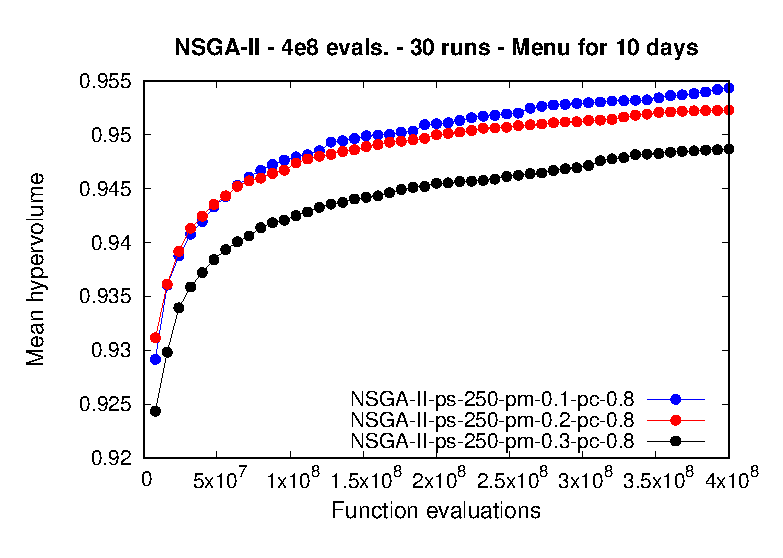
\includegraphics[width=1.0\linewidth]{../references/meanHV_Evolution_NSGA2_days_10.eps}
  \label{fig:sfig1}
    \caption{Evolution of the average HV value for every NSGA-II configuration tested in \cite{Miranda2018}.}
\end{subfigure}%
\begin{subfigure}{.5\textwidth}
  \centering
  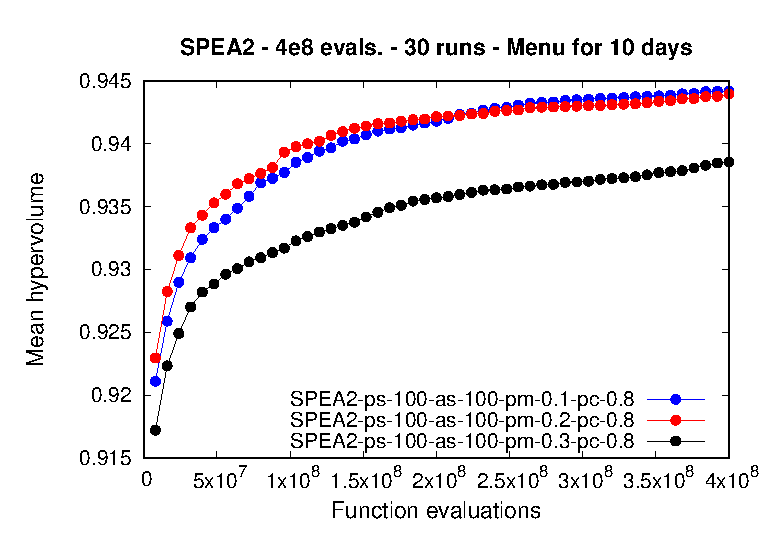
\includegraphics[width=1.0\linewidth]{../references/meanHV_Evolution_SPEA2_days_10.eps}
  \label{fig:sfig2}
  \caption{Evolution of the average HV value for every SPEA-2 configuration tested in \cite{Miranda2018}.}
\end{subfigure}
\centering
\begin{subfigure}{.9\textwidth}
  \centering
  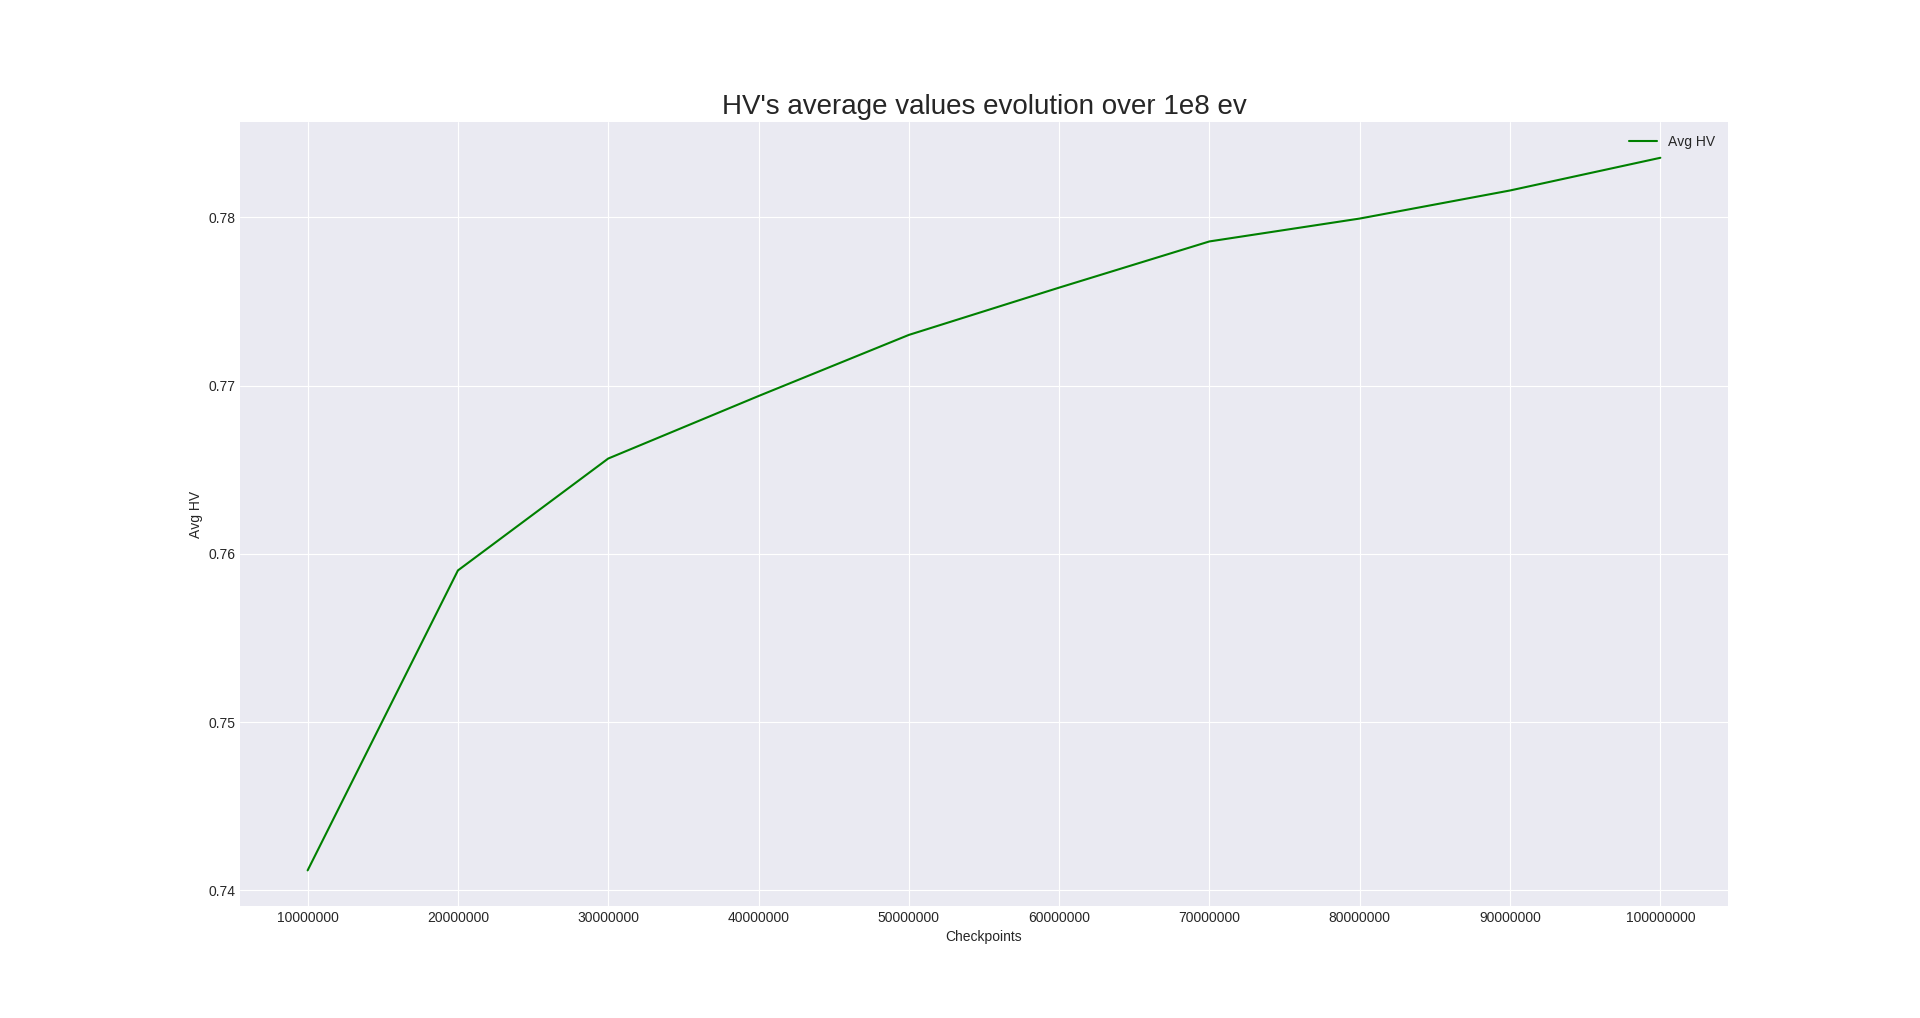
\includegraphics[width=1.0\linewidth]{../experiments/plots/avgHV_evolution_10_days.png}
  \caption{Evolution of the average HV value for a 10-days MPP of the best MOEA/D configuration found.}
\end{subfigure}
\caption{Evolution of the average HV value for a 10-days MPP extracted from\cite{Miranda2018}.}
\label{fig:previous_HV_10}
\end{figure}


\begin{figure}[H]
\begin{subfigure}{.5\textwidth}
  \centering
  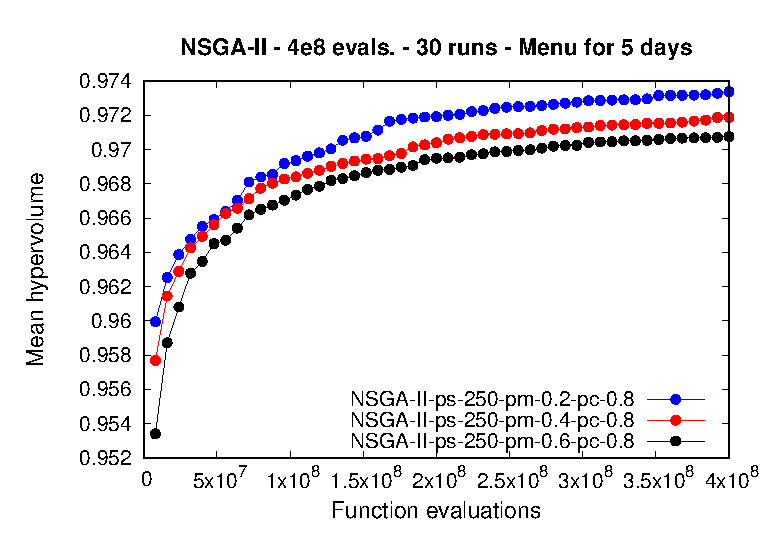
\includegraphics[width=1.0\linewidth]{../references/meanHV_Evolution_NSGA2_days_5.eps}
  \label{fig:sfig1}
    \caption{Evolution of the average HV value for every NSGA-II configuration tested in \cite{Miranda2018}.}
\end{subfigure}%
\begin{subfigure}{.5\textwidth}
  \centering
  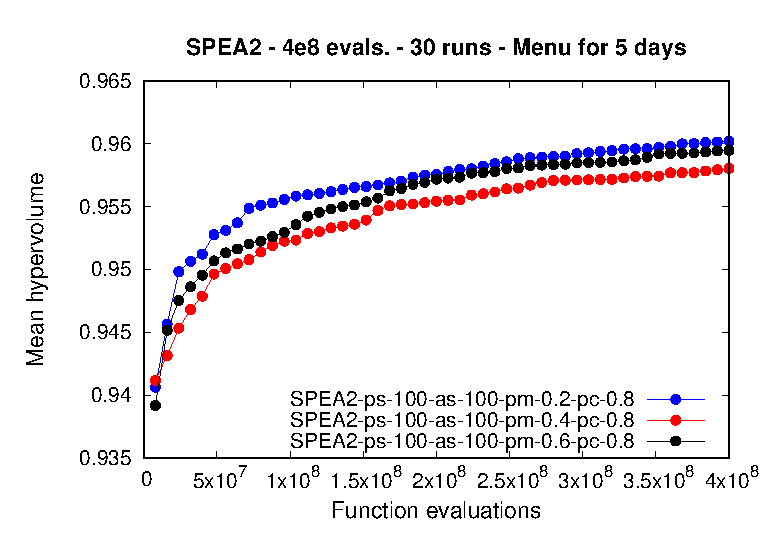
\includegraphics[width=1.0\linewidth]{../references/meanHV_Evolution_SPEA2_days_5.eps}
  \label{fig:sfig2}
  \caption{Evolution of the average HV value for every SPEA-2 configuration tested in \cite{Miranda2018}.}
\end{subfigure}
\centering
\begin{subfigure}{.9\textwidth}
  \centering
  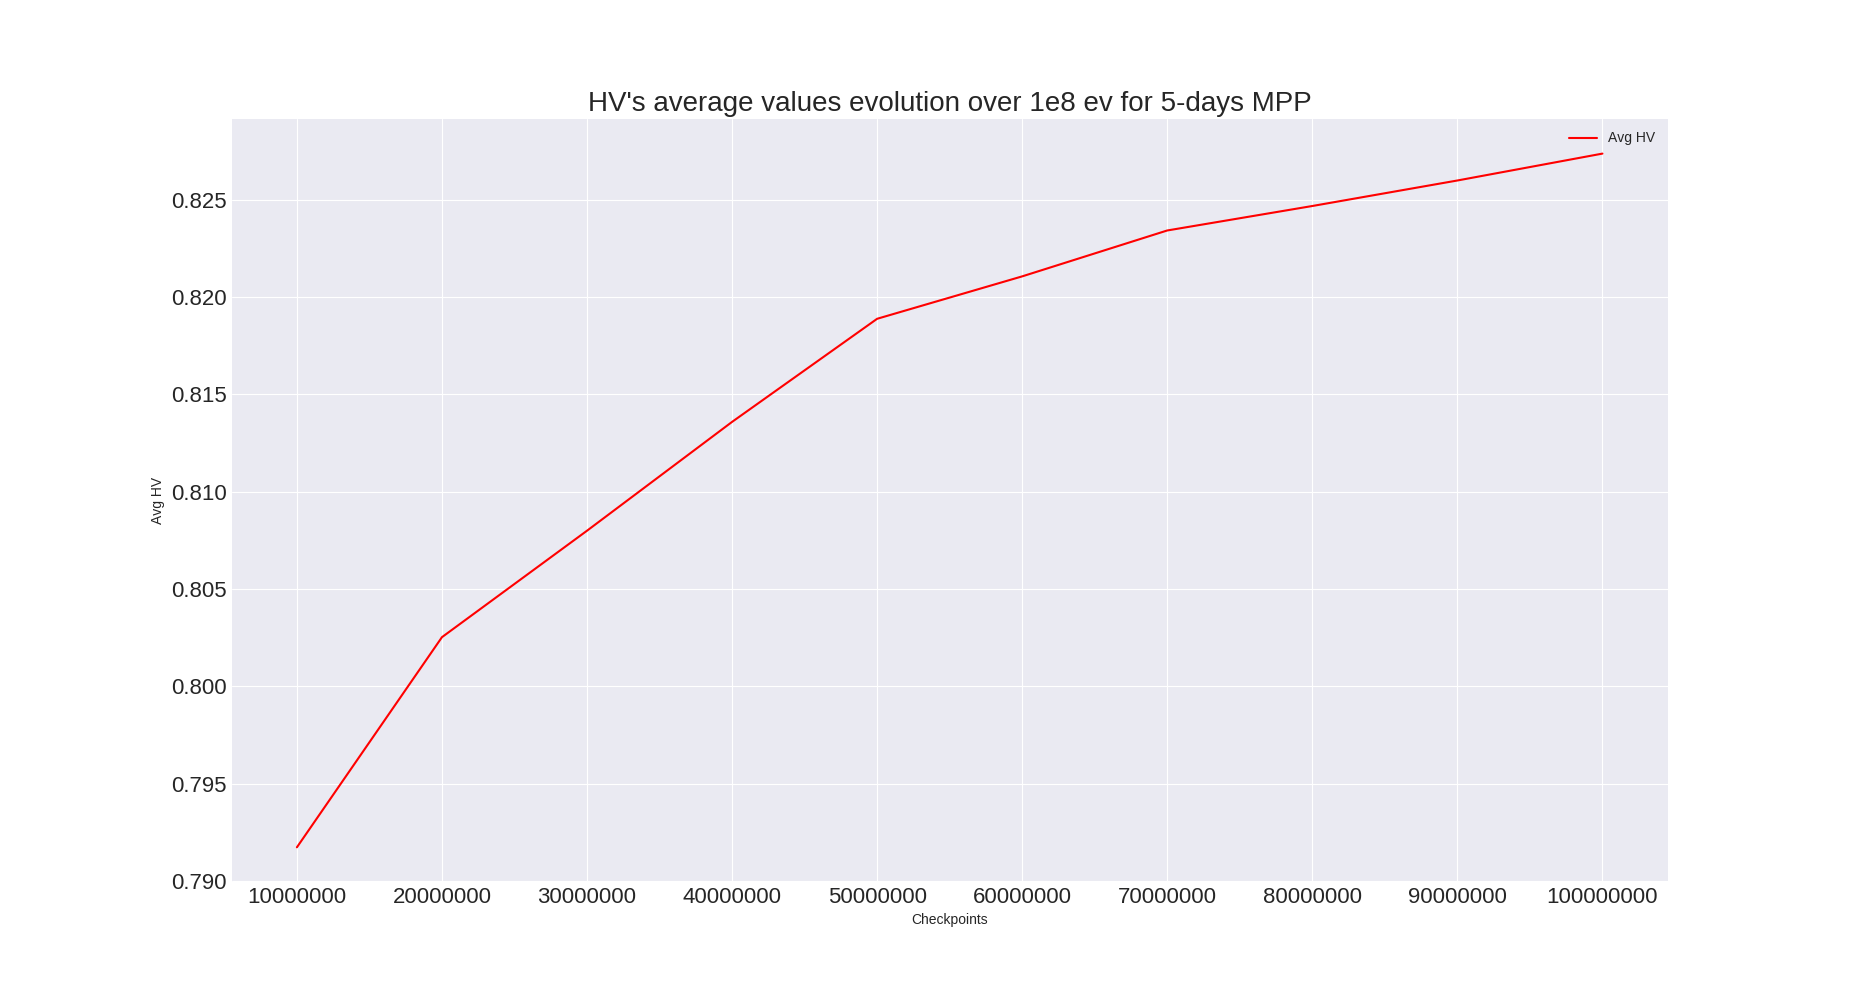
\includegraphics[width=1.0\linewidth]{../experiments/plots/avgHV_evolution_5_days.png}
  \caption{Evolution of the average HV value for a 5-days MPP of the best MOEA/D configuration found.}
\end{subfigure}
\caption{Evolution of the average HV value for a 5-days MPP extracted from\cite{Miranda2018}.}
\label{fig:previous_HV_5}
\end{figure}





\begin{figure}[H]
\begin{subfigure}{.5\textwidth}
  \centering
  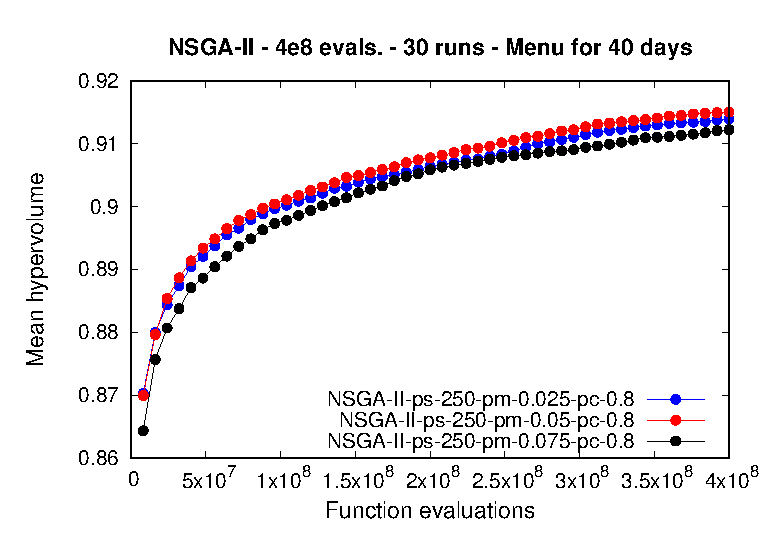
\includegraphics[width=1.0\linewidth]{../references/meanHV_Evolution_NSGA2_days_40.eps}
  \label{fig:sfig1}
    \caption{Evolution of the average HV value for every NSGA-II configuration tested in \cite{Miranda2018}.}
\end{subfigure}%
\begin{subfigure}{.5\textwidth}
  \centering
  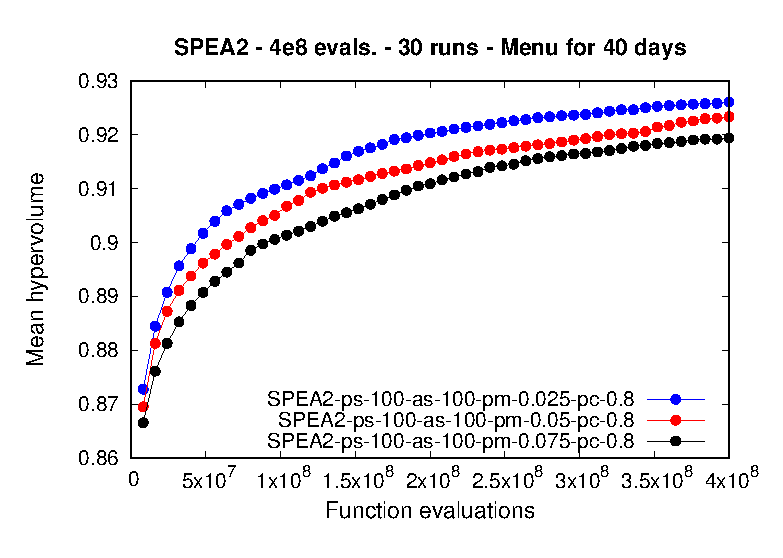
\includegraphics[width=1.0\linewidth]{../references/meanHV_Evolution_SPEA2_days_40.eps}
  \label{fig:sfig2}
  \caption{Evolution of the average HV value for every SPEA-2 configuration tested in \cite{Miranda2018}.}
\end{subfigure}
\centering
\begin{subfigure}{.9\textwidth}
  \centering
  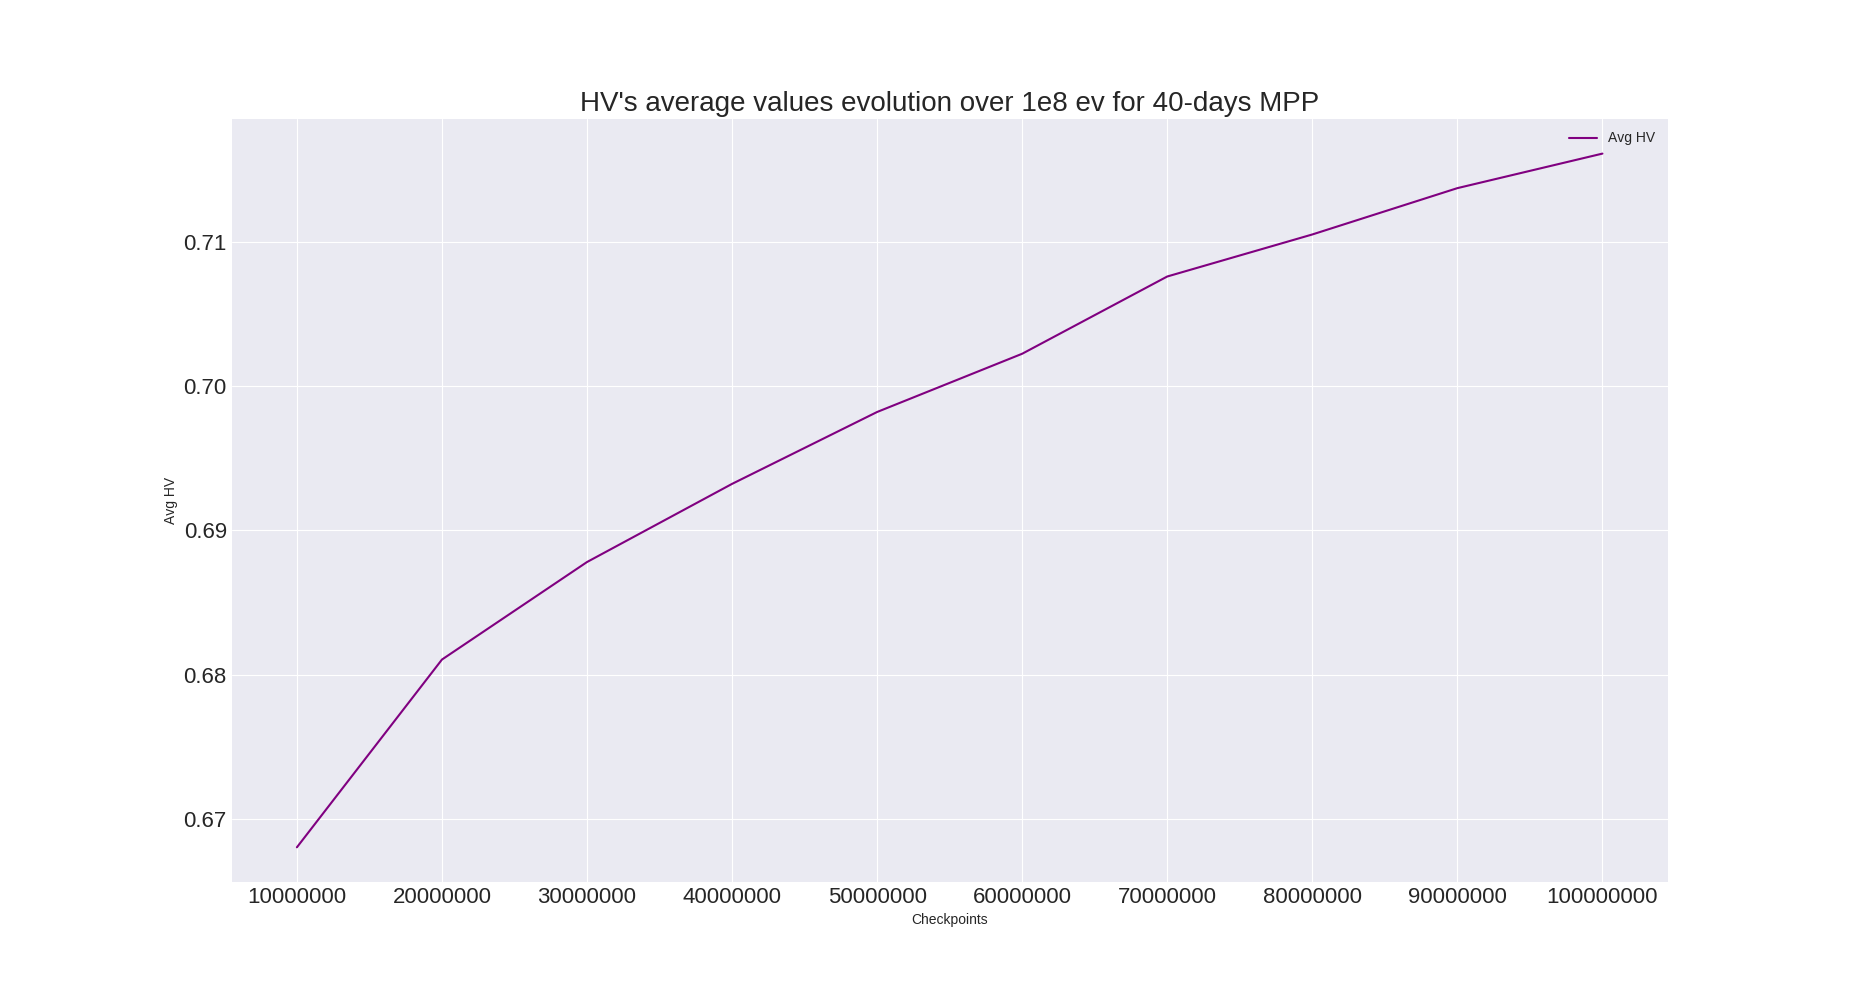
\includegraphics[width=1.0\linewidth]{../experiments/plots/avgHV_evolution_40_days.png}
  \caption{Evolution of the average HV value for a 40-days MPP of the best MOEA/D configuration found.}
\end{subfigure}
\caption{Evolution of the average HV value for a 40-days MPP extracted from\cite{Miranda2018}.}
\label{fig:previous_HV_40}
\end{figure}


%%%%%%%%%%%%%%%%%%%%%%%%%%%%%%%%%%%%%%%%%%%%%%%%%%%%%%%%%%%%%%%%%%%%%
Besides, Pareto Front representations of the final results are shown at Figures \ref{fig:front_comp_1}, \ref{fig:front_comp_2} \ref{fig:front_comp_3}. Although MOEA/D obtains menu plans with less degree of repetition, the total cost of the menu plan is slightly higher compared with the results obtained by NSGA-II and SPEA-2 with almost the same degree of repetition for 5-days, 10-days and 40-days MPP instances. These results are more than acceptable considering that MOEA/D performs four times less evaluations that NSGA-II and SPEA-2 in the experimental evaluation done in \cite{Miranda2018}.
\begin{figure}[H]
\begin{subfigure}{.5\textwidth}
  \centering
  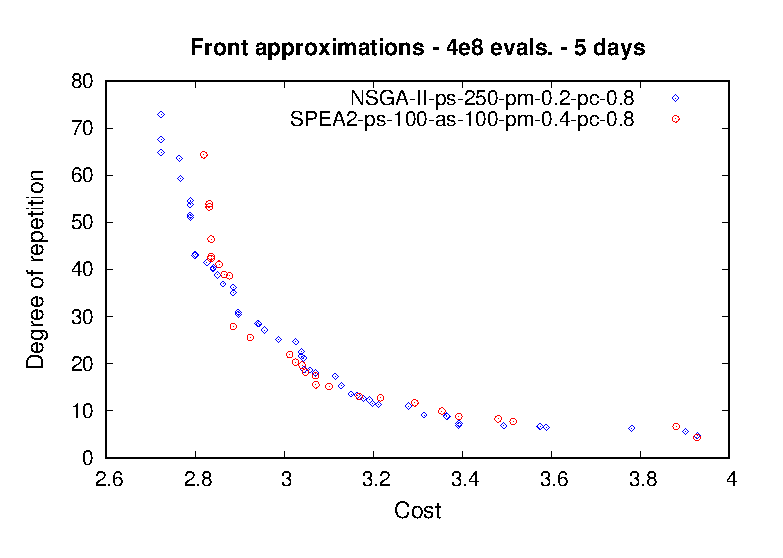
\includegraphics[width=1.0\linewidth]{../references/fronts_5days.eps}
\end{subfigure}%
\begin{subfigure}{.5\textwidth}
  \centering
  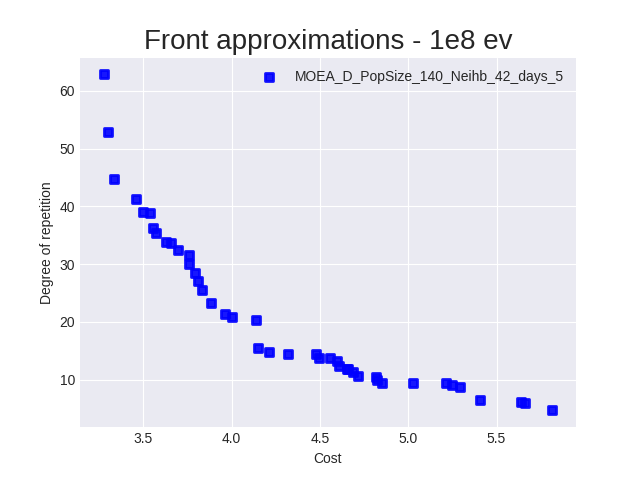
\includegraphics[width=1.0\linewidth]{../experiments/plots/fronts/5_days/MOEA_D_PopSize_140_Neihb_42_days_5_6.png}
\end{subfigure}
\caption{Front approximation comparison between NSGA-II and SPEA-2 at 4e8 evaluations against best MOEA/D configuration found so far at 1e8 evaluations facing a 5-days MPP.}
\label{fig:front_comp_1}
\end{figure}

\begin{figure}[H]
\begin{subfigure}{.5\textwidth}
  \centering
  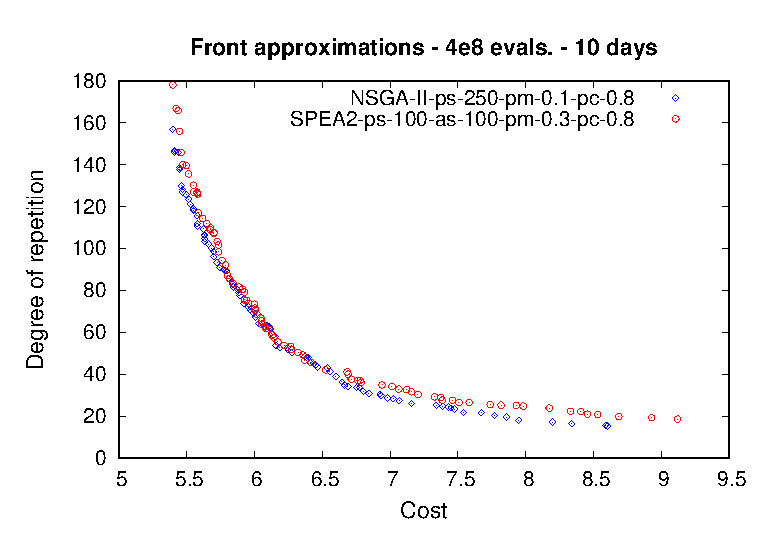
\includegraphics[width=1.0\linewidth]{../references/fronts_10days.eps}
\end{subfigure}%
\begin{subfigure}{.5\textwidth}
  \centering
  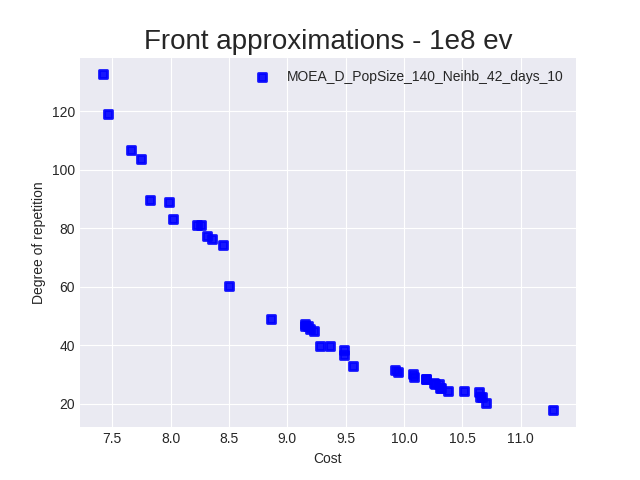
\includegraphics[width=1.0\linewidth]{../experiments/plots/fronts/10_days/MOEA_D_PopSize_140_Neihb_42_days_10_10.png}
\end{subfigure}
\caption{Front approximation comparison between NSGA-II and SPEA-2 at 4e8 evaluations against best MOEA/D configuration found so far at 1e8 evaluations facing a 10-days MPP.}
\label{fig:front_comp_2}
\end{figure}


\begin{figure}[H]
\begin{subfigure}{.5\textwidth}
  \centering
  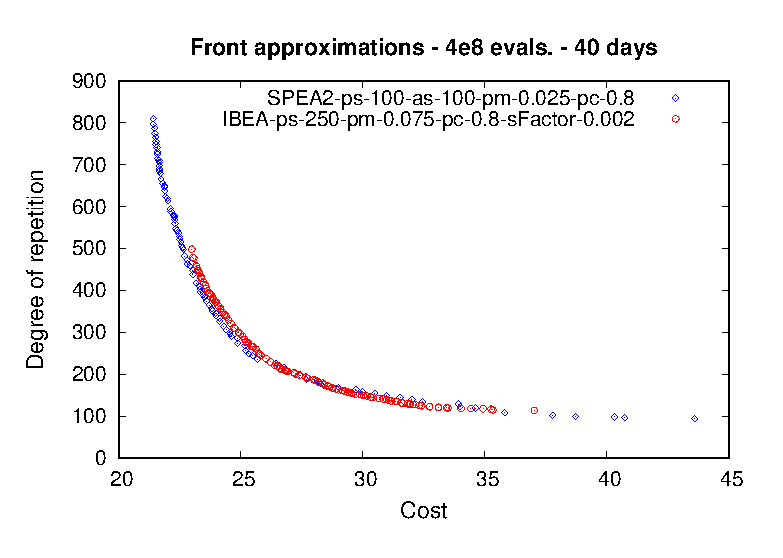
\includegraphics[width=1.0\linewidth]{../references/fronts_40days.eps}
\end{subfigure}%
\begin{subfigure}{.5\textwidth}
  \centering
  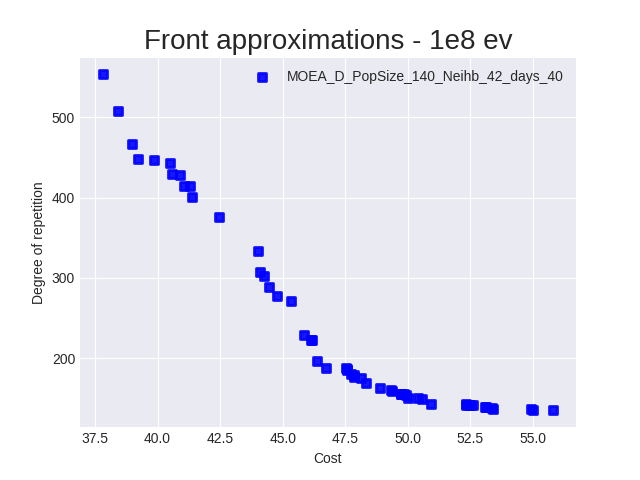
\includegraphics[width=1.0\linewidth]{../experiments/plots/fronts/40_days/MOEA_D_PopSize_140_Neihb_42_days_40_10.png}
\end{subfigure}
\caption{Front approximation comparison between NSGA-II and SPEA-2 at 4e8 evaluations against best MOEA/D configuration found so far at 1e8 evaluations facing a 40-days MPP.}
\label{fig:front_comp_3}
\end{figure}

Lastly, due to the fact that the previous work and this experimental evaluation was done with the same framework and run in the same system, an reliable elapsed time comparison between the different algorithms can be made. The following Table \ref{table:time} shows the average time in hours for 25 independent runs for every compared algorithm. As results show, NSGA-II totally outperforms both SPEA-2 and MOEA/D for 5, 10, and 20-days MPP instances. However, surprisingly MOEA/D obtains quite faster but low quality results than NSGA-II and SPEA-2 for 40-days MPP.
 
% Please add the following required packages to your document preamble:
% \usepackage{graphicx}
\begin{table}[H]
\centering
\begin{tabular}{cc}
\hline
\multicolumn{1}{l}{\textbf{5-days MPP}} & \multicolumn{1}{l}{} \\ \hline
\multicolumn{1}{l}{Algorithm} & \multicolumn{1}{l}{Avg Elapsed Time (hours)} \\ \hline
NSGA-II & 5.579 \\
SPEA-2 & 7.734 \\
MOEA/D & 11.047 \\ \hline
\multicolumn{1}{l}{10-days MPP} & \multicolumn{1}{l}{} \\ \hline
\multicolumn{1}{l}{Algorithm} & \multicolumn{1}{l}{Avg Elapsed Time (hours)} \\ \hline
NSGA-II & 6.838 \\
MOEA/D & 8.549 \\
SPEA-2 & 8.855 \\ \hline
\multicolumn{1}{l}{20-days MPP} & \multicolumn{1}{l}{} \\ \hline
\multicolumn{1}{l}{Algorithm} & \multicolumn{1}{l}{Avg Elapsed Time (hours)} \\ \hline
NSGA-II & 9.269 \\
MOEA/D & 10.724 \\
SPEA-2 & 11.554 \\ \hline
\multicolumn{1}{l}{40-days MPP} & \multicolumn{1}{l}{} \\ \hline
\multicolumn{1}{l}{Algorithm} & \multicolumn{1}{l}{Avg Elapsed Time (hours)} \\ \hline
MOEA/D & 8.463 \\
NSGA-II & 13.976 \\
SPEA-2 & 16.312
\end{tabular}%
\caption{MOEA/D performance comparison against best results of NSGA-II and SPEA-2 from \cite{Miranda2018} with different MPP sizes.}
\label{table:time}
\end{table}